\section{Grafi}
I grafi sono una formalizzazione della connessione e relazione tra oggetti.
Un grafo $G$ è una coppia $V,E$ dove $V$ è un insieme finito di \emph{vertici (o nodi)}
ed $E$ è un sottoinsieme di $V \cdot V$ segmenti detti \emph{archi, lati o spigoli}.
\begin{equation*}
    G = (V, E) \quad \quad E \subseteq V \cdot V
\end{equation*}
I grafi possono essere \emph{orientati} o \emph{non orientati}. Nel primo caso
gli archi rappresentano una relazione simmetrica, cioè valida tra due nodi in entrambe
le direzioni, nel secondo caso solo in una direzione.\\
Vediamo ora una serie di termini legati ai grafi.
Dato un generico arco $(x, y) \in E$ in un grafo con vertici $V$:
\begin{itemize}
    \item Un arco è \textbf{\emph{incidente}} su due vertici
    \item Se un arco \textbf{\emph{esce}} da $x$ ed \textbf{\emph{entra}} in $y$, allora $y$ è \textbf{\emph{adiacente}} ad $x$
    \item I \textbf{\emph{vicini}} di un vertice sono i vertici adiacenti ad esso
    \item Il \textbf{\emph{grado}} di un vertice è il numero di archi incidenti al vertice
    \item Un \textbf{\emph{cammino}} da $x$ a $y$ è una sequenza di vertici collegati da archi appartenenti al grafo in cui il vertice di partenza è $x$ e quello di arrivo $y$
    \item La \textbf{\emph{lunghezza del cammino}} è il numero di archi del cammino
    \item $y$ è \textbf{\emph{raggiungibile}} da $x$ se esiste un cammino da $x$ a $y$
    \item Un \textbf{\emph{cammino semplice}} non contiene vertici ripetuti
    \item Un \textbf{\emph{ciclo}} è un cammino da $x$ a $x$
    \item In un \textbf{\emph{ciclo semplice}} è ripetuto solo il vertice iniziale, alla fine 
    \item Una \textbf{\emph{catena}} tra $x$ e $y$ è una sequenza in cui non rispetto l'orientamento degli archi
    \item Un \textbf{\emph{circuito}} è una catena da $x$ a $x$
    \item Un grafo è \textbf{\emph{connesso}} quando per ogni coppia di vertici esiste una catena
    \item Un grafo è \textbf{\emph{fortemente connesso}} quando per ogni coppia di vertici esiste un cammino
    \item Un \textbf{\emph{sottografo}} è un grafo in cui prendo solo alcuni vertici e alcuni archi 
    \item Un \textbf{\emph{sottografo indotto}} è un grafo in cui prendo solo alcuni vertici e tutti i loro archi incidenti
    \item Una \textbf{\emph{componente fortemente connessa}} è un sottografo indotto fortemente connesso massimale
    \item Un \textbf{\emph{circuito hamiltoniano}} è un circuito che passa per ogni vertice del grafo una e una sola volta
    \item Un \textbf{\emph{circuito euleriano}} è un circuito che attraversa ogni arco del grafo una e una sola volta
    \item Un \textbf{\emph{multigrafo}} è un grafo in cui 2 vertici sono sollegati da più di un arco 
\end{itemize}

A questo punto possiamo dare la definizione formale di albero:
\begin{center}
    Un albero è un grafo non orientato, connesso e privo di cicli.
\end{center}

Alcuni teoremi riguardanti i grafi:
\begin{enumerate}
    \item esiste un circuito euleriano se e solo se ogni vertice ha grado pari
    \item è sempre possibile suddividere un grafo in componenti fortemente connesse
    \item Se un grafo è un albero allora il numero di vertici è uguale al numero di archi +1
    \item Se un grafo è non orientato e connesso, allora, se il numero di vertici è = al numero di archi +1, è un albero
    \item Un albero  
\end{enumerate}

\subsection*{Albero di supporto o ricoprente (Spanning tree)}
Dato un grafo $G = (V,E)$ orientato non connesso, un albero ricoprente di $G$
è un albero $G' = (V', E')$ con $V' = V$ ed $E' \subseteq E$.\\
Una \textbf{\emph{cricca}} è un grafo non orientato completo, ovvero in cui c'è un arco per ogni coppia di vertici  
\clearpage

\subsection{Rappresentazione di grafi}
Vediamo ora alcuni metodi per rappresentare i grafi. La rappresentazione migliore dipende dai casi di utilizzo.
\subsubsection{Lista di archi}
Possiamo rappresentare gli archi come un elenco contenente le coppie di vertici
che l'arco collega. Vale anche per i grafi orientati, ricordando che la posizione del 
nodo all'interno della coppia rappresenta l'orientamento dell'arco.
Questa struttura è comoda per vedere i vertici di un arco ma è scomoda per 
ricostruire la forma del grafo, per seguire un cammino o se voglio sapere a cosa è
collegato direttamente un vertice. In quest'ultimo caso infatti dovrei attraversare tutta la struttura.
Lo spazio complessivo utilizzato è $O(n+m)$
\begin{figure}[h]
    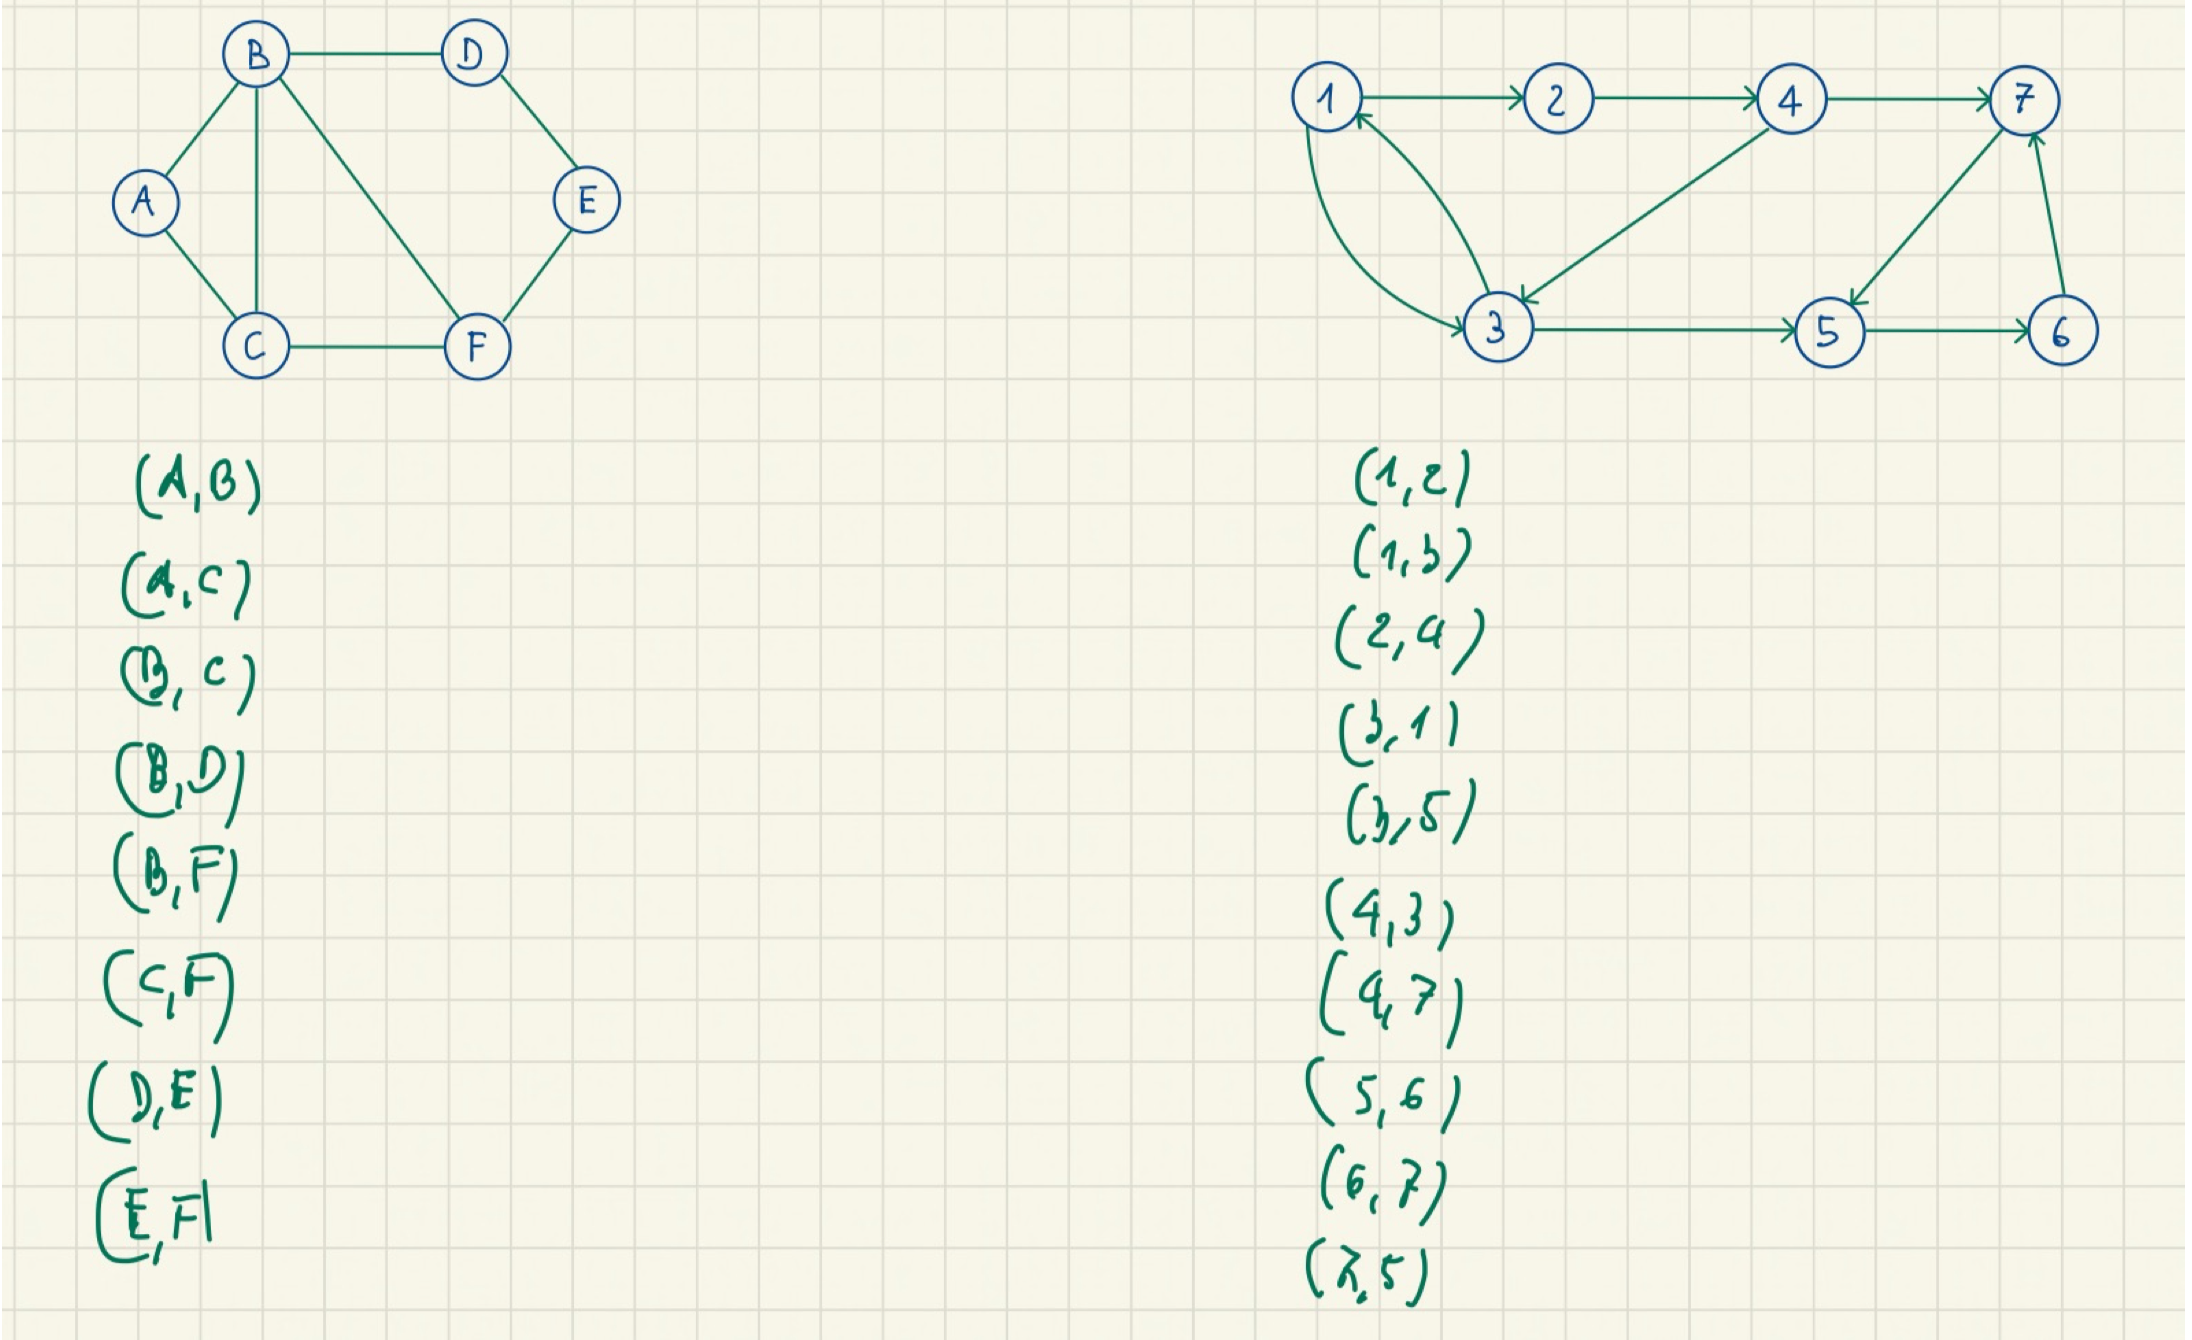
\includegraphics[width=\textwidth]{lista_archi.png}
\end{figure}
\clearpage

\subsubsection{Lista di adiacenza}
Struttura principale basata sui vertici. Per ogni vertice esiste la lista dei vertici adiacenti.
Ogni arco è rappresentato due volte, quindi lo spazio occupato è $2m$ (solo dai nodi).
Questa struttura è comoda per gli archi uscenti da ogni nodo ma se devo trovare gli archi 
entranti ad un nodo devo passare tutta la struttura. Inoltre non abbiamo informazioni esplicite sugli archi.
Lo spazio complessivo utilizzato è $O(n+m)$
\begin{figure}[h]
    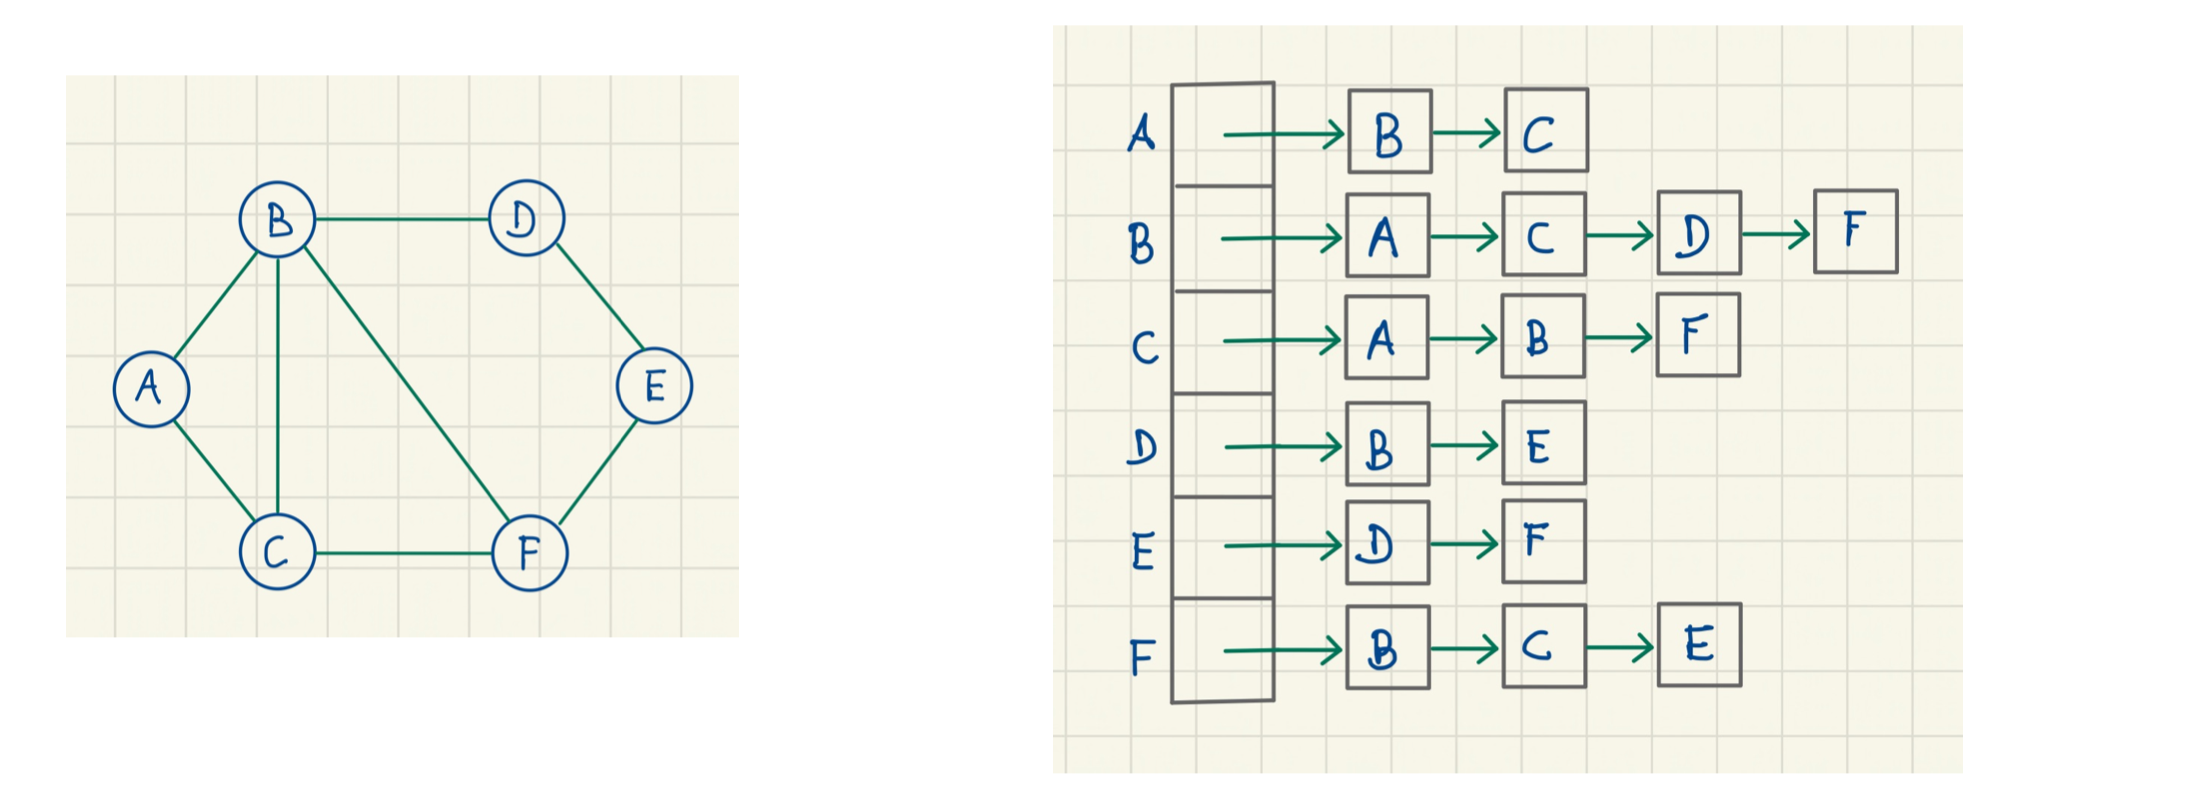
\includegraphics[width=\textwidth]{lista_adiacenza.png}
\end{figure}

\subsubsection{Lista di incidenza}
Rimpiazziamo le liste dei vertici delle liste di adiacenza con delle liste di archi,
tornando a usare strutture come nella lista di archi. Rimane il problema citato precedentemente 
sugli archi entranti.
Lo spazio complessivo utilizzato è $O(n+m)$
\begin{figure}[h]
    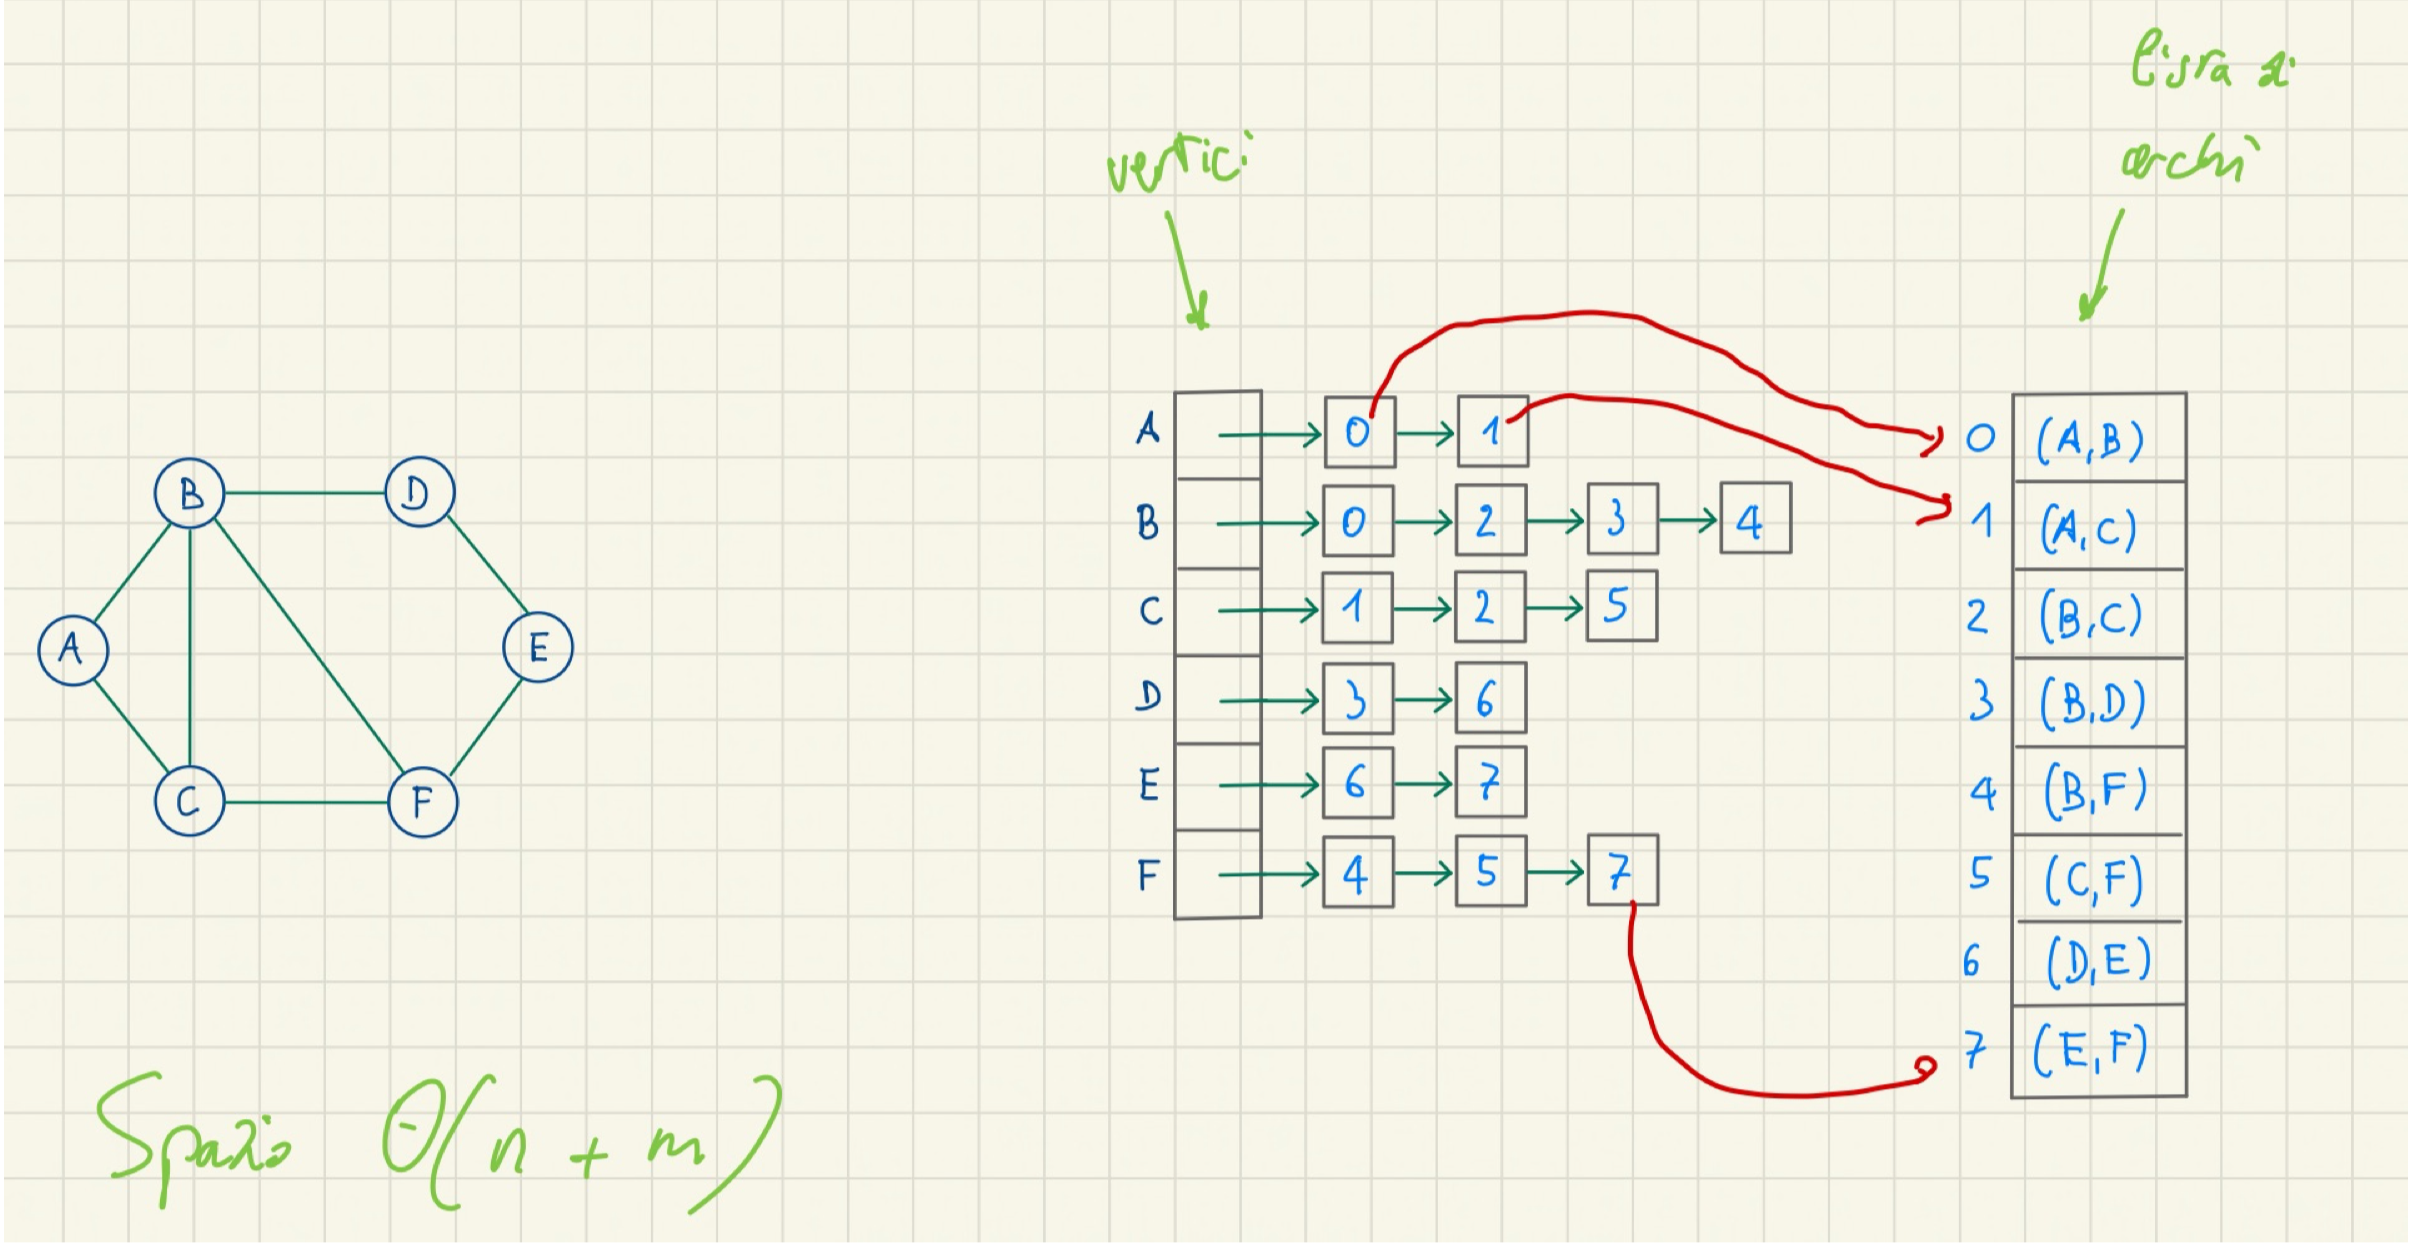
\includegraphics[width=\textwidth]{lista_incidenza.png}
\end{figure}
\clearpage

\subsubsection{Matrice di adiacenza}
Si tratta di una matrice quadrata di 0 e 1 dove gli indici sono i vertici del grafo.\\
$M[u,v] = 1$ se e solo se $(u, v) \in E$.
Un grafo non orientato genera una matrice simmetrica. Osservando la matrice 
è possibile notare che possiamo vedere anche gli archi entranti leggendo le colonne.
Lo spazio complessivo utilizzato è $O(n^2)$. Tale spazio è molto diverso da 
$O(n+m)$? Dipende dal numero di archi.
Si può dimostrare che, per ogni $k > 0$:
\begin{center}
    $M^k[u,v] = 1$ sse $V^{n-1}_{k=0}M^k$ "sommatoria" di OR
\end{center}
Nella matrice risultante, se c'è un 1 in una determinata posizione significa che esiste un cammino.
Quindi, in un grafo fortemente connesso, la matrice risultante sarà composta solo da 1.
\begin{figure}[h]
    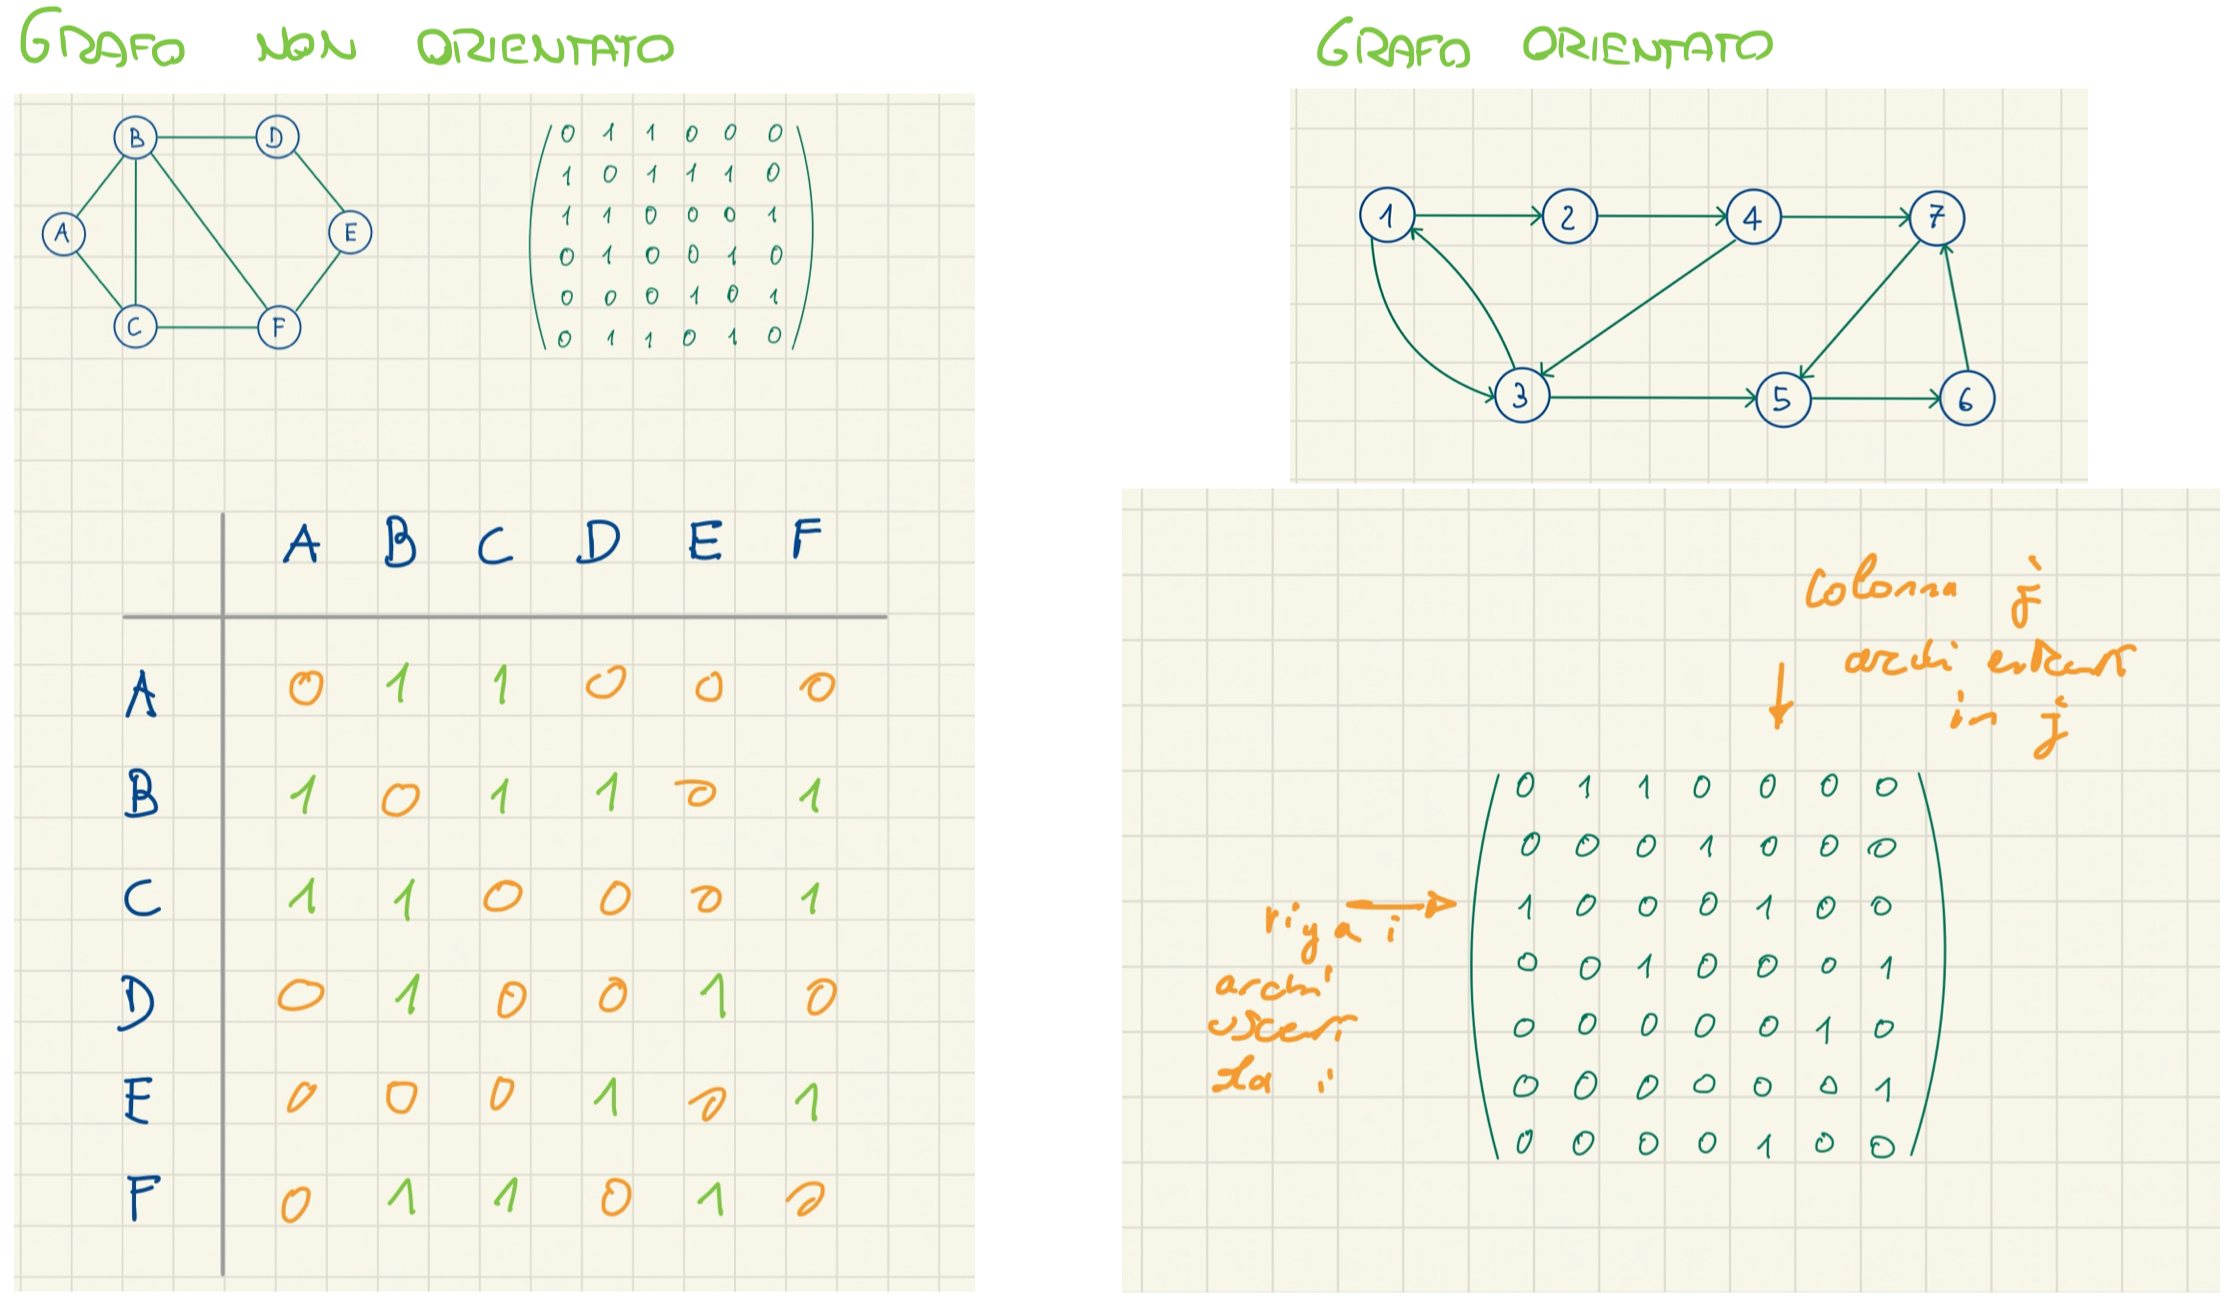
\includegraphics[width=\textwidth]{matrice_adiacenza.png}
\end{figure}
\clearpage 

\subsubsection{Matrice di incidenza}
Abbiamo una riga per ogni vertice e una colonna per ogni arco. Nei grafi non orientati metto 1 quando c'è un 
collegamento diretto, nei grafi orientati ho 1 quando c'è un arco uscente e -1 quando
c'è un arco entrante.
Questo sistema ci permette di risparmiare un po' di spazio mantenendo l'informazione
su archi uscenti ed entranti per grafi orientati.
Lo spazio complessivo è $O(n \cdot m)$\\
\textbf{N.B.} Ogni colonna contiene un 1 e un -1, quindi la somma algebrica di ogni colonna è pari a 0.
\begin{figure}[h]
    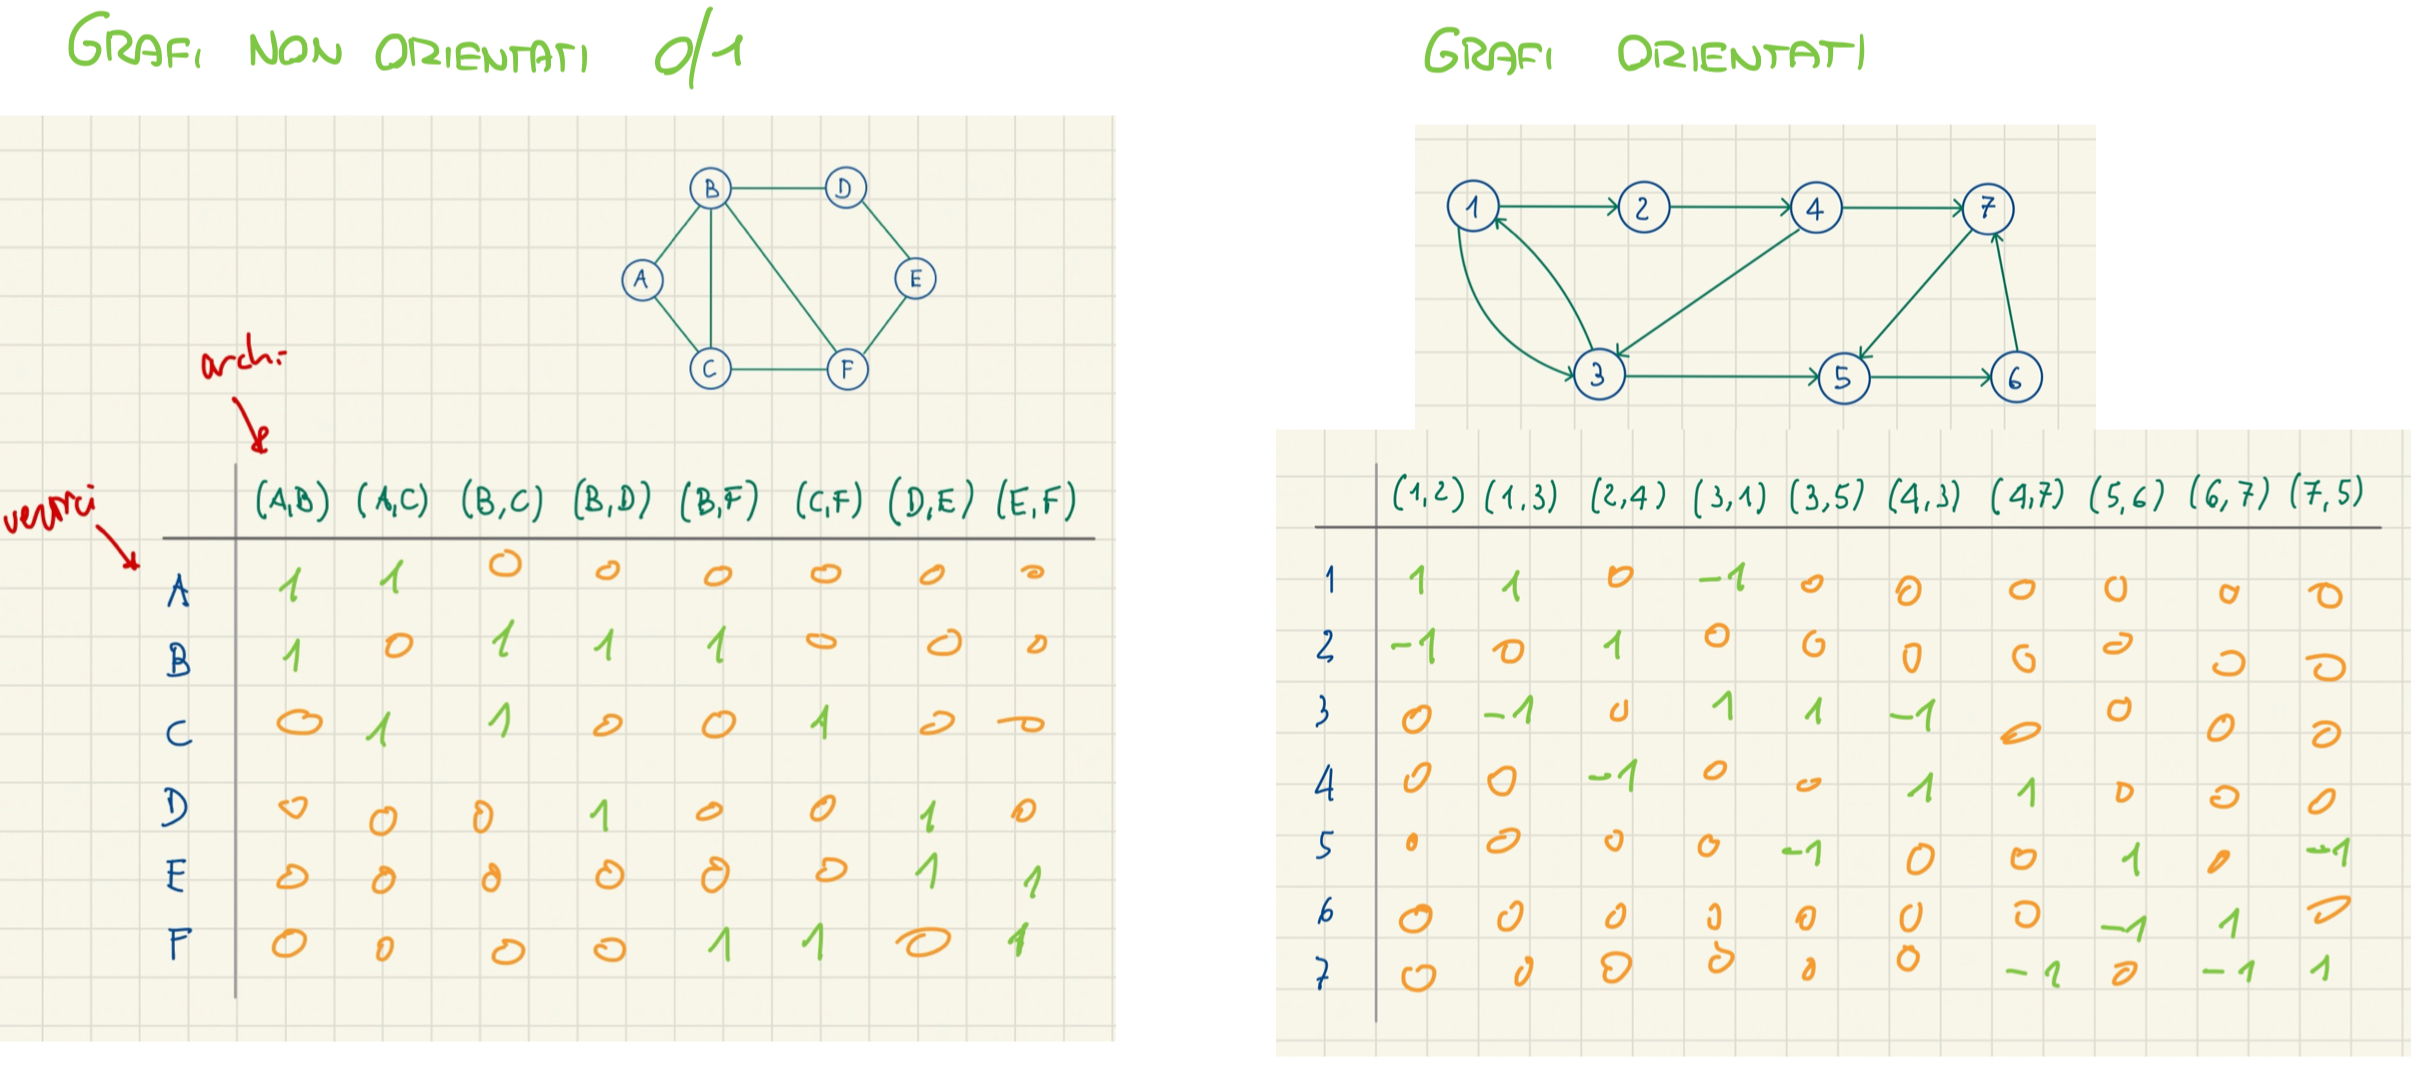
\includegraphics[width=\textwidth]{matrice_incidenza.png}
\end{figure}
\clearpage


\subsection{Attraversamento di grafi}
Esistono diverse strategie per attraversare un grafo. Noi vedremo le visite in 
ampiezza e in profondità per grafi connessi e non orientati. I concetti di visità in ampiezza 
e in profondità sono gli stessi visti per gli alberi con radice.
Il tempo impiegato dall'algoritmo dipende dalla struttura dati utilizzata per rappresentare il grafo.\\

\noindent $G = (V,E)$ grafo connesso non orientato,\\
$s \in V$ vertice di partenza.
\subsubsection{Visita in ampiezza}
Questo algoritmo visita il grafo in ampiezza e crea un albero di supporto basato sul grafo 
dato in ingresso.\\
\begin{figure}[h]
    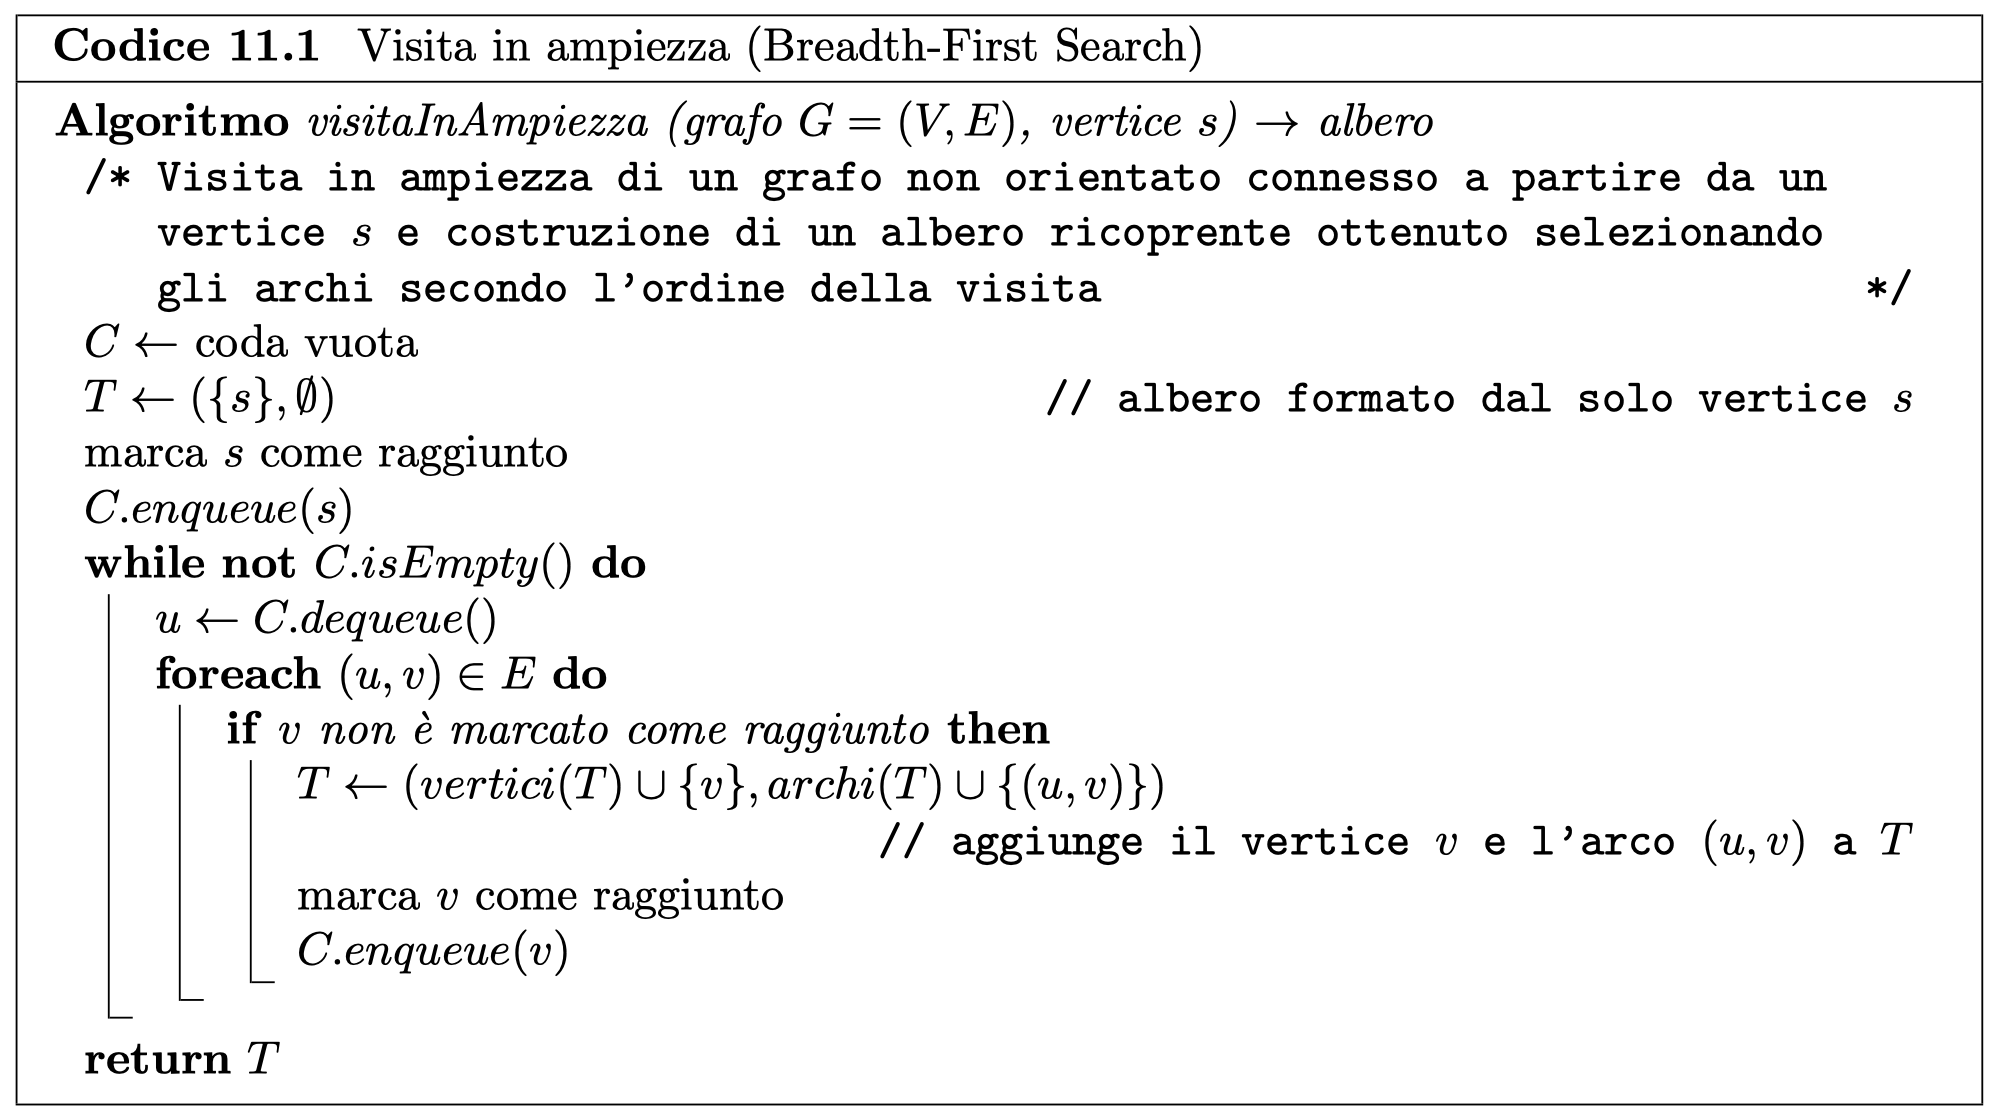
\includegraphics[width=\textwidth]{visita_ampiezza_grafi.png}
\end{figure}

\begin{tabular}{|l|c|}
    \hline
    \textbf{Lista di archi} & $O(n \cdot m)$ \\
    \hline
    \textbf{Lista di adiacenza} & $O(n + m)$ \\
    \hline
    \textbf{Lista di incidenza} & $O(n + m)$ \\
    \hline
    \textbf{Matrice di adiacenza} & $O(n^2)$ \\
    \hline
    \textbf{Matrice di incidenza} & $O(n \cdot m)$ \\
    \hline
\end{tabular}
\clearpage

\subsubsection{Visita in profondità}
Si parte da un vertice e si cerca di esplorare il più possibile partendo da ogni 
nodo in cui entriamo di volta in volta, finchè non posso più muovermi. A quel punto 
torno indietro finchè non trovo la prima strada che posso percorrere. Si va avanti fino a che 
non ho attraversato tutto il grafo. L'implementazione avviene tramite una pila o ricorsivamente (meglio la seconda alternativa).
I tempi sono gli stessi visti per la visita in ampiezza.
\begin{figure}[h]
    \includegraphics[width=\textwidth]{visita_profondità_grafi.png}
\end{figure}

\clearpage

